\paragraph{\trGenerator{}。}\label{sub:milnor-fibre-generators}
对任意的 $n\ge 1$ 与 $m\ge 2$，考虑函数 $\Psi(x)=p(x_0)+x_1^2+\cdots+x_n^2\colon\CC^{n+1}\to\CC$，其中 $p$ 是某个 $m+1$ 次的多项式。我们将关注于
\begin{equation*}
X^n_m=\Psi^{-1}(w),
\end{equation*}
其中 $w$ 是 $\Psi$ 的一个\trRegularValue。这是一个\trSmooth\trHypersurface，因而特别地是一个\trCanonical{}丛平凡的仿射代数 $n$-簇。我们不取它的一个适当的\trCompact{}部分，而是（本着注记 19.5 的精神）宁愿与 $X^n_m$ 本身打交道：为其配备上 $\CC^{n+1}$ 上\trFlat\trKaehler{}形式的限制、它的标准 1-形式原函数，以及二次复\trVolume{}形式 $\eta^2$——后者满足 $\eta\wedge d\Psi=dx_0\wedge\cdots\wedge dx_n$。在相差一个\trExact{}辛\trIsomorphism{}的意义下，$X^n_m$ 从而与 $p$ 和 $w$ 的选取无关，从而 $\scr{F}(X^n_m)$ 亦然。
设 $p$ 是\trGeneric{}的，也就是说它的\trCriticalPoint{}都是\trNondegenerate{}的。在这种情形下，经过一些适当的技术调整之后，可以把 $\Psi$ 视为一个\trLefschetzFibration。以适当的方式选取\trVanishingPath{}的一组基，便得到\trVanishingCycle{}的一组基 $(V_1,\ldots,V_m)$，它们的（两两\trTransverse{}的）相交情况为：
\begin{equation}\label{eq:intersection-matrix}
|V_i\cap V_j|=
\begin{cases}
1 & \text{当 } |i-j|=1 \text{ 时，} \\
0 & \text{当 } |i-j|\ge 2 \text{ 时。}
\end{cases}
\end{equation}
把它们\trLift{}为\trLagrange\trBrane{}$(V_1^\#,\ldots,V_m^\#)$，并取相伴的\trFullSubcategory{}$\scr{F}^n_m\subset\scr{F}(X^n_m)$。
\trCohomology{}层面（\trDonaldson--\trFukaya）的\trCategory{}$H(\scr{F}^n_m)$ 可以容易地算出，只需用到 \eqref{eq:intersection-matrix} 以及\trFloerCohomology{}的一般性质。循着 [85]，我们以\textbf{\trQuiver{}代数}（quiver algebra）的语言来陈述这一结果。考虑\trGraded{}\textbf{\trQuiver}（quiver）
\begin{equation}\label{eq:graded-quiver}
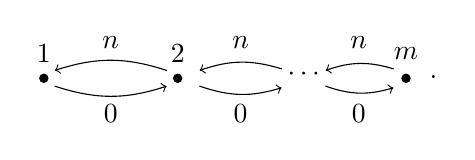
\begin{tikzpicture}[line cap=round,line join=round]
\fill (0,0) circle (1.7pt);
\node at (0,0.32) {$1$};
\fill (1.7,0) circle (1.7pt);
\node at (1.7,0.32) {$2$};
\node at (3.3,0.05) {$\cdots$};
\fill (4.6,0) circle (1.7pt);
\node at (4.6,0.32) {$m$};
\node at (4.95,0.02) {$.$};
\draw[->] (1.56,0.1) to[bend right=18] (0.14,0.1);
\node at (0.85,0.45) {$n$};
\draw[->] (0.14,-0.1) to[bend right=18] (1.56,-0.1);
\node at (0.85,-0.45) {$0$};
\draw[->] (3.02,0.12) to[bend right=18] (1.98,0.1);
\node at (2.5,0.45) {$n$};
\draw[->] (1.98,-0.1) to[bend right=18] (3.02,-0.12);
\node at (2.5,-0.45) {$0$};
\draw[->] (4.44,0.12) to[bend right=18] (3.58,0.1);
\node at (4.0,0.45) {$n$};
\draw[->] (3.58,-0.1) to[bend right=18] (4.44,-0.12);
\node at (4.0,-0.45) {$0$};
\end{tikzpicture}
\end{equation}
一般地说，对任何一个这样的\trQuiver{}都可以配上一个\trGraded{}结合代数，称为\textbf{\trPathAlgebra}（path algebra）。在所讨论的这个例子中，\trPathAlgebra{}的元素是基本表达式 $(i_l,\ldots,i_0)$（$l\ge 0$）的\trLinear{}组合，其中 $i_j\in\{1,\ldots,m\}$，并且 $|i_{j+1}-i_j|=1$。这种基元素的\trDegree{}是 $n$ 乘以那些使 $i_{j+1}=i_j-1$ 的 $j$ 的个数。乘法由路径的\trComposition{}给出，例如 $(i+2,i+1)\,(i+1,i)=(i+2,i+1,i)$。特别地，长度为零的路径 $(i)$ 是两两\trOrthogonal{}的\trIdempotent。它们的存在使\trPathAlgebra{}成为\trSemisimple{}环 $R_m\cong\KK^m$ 上的一个代数。
令 $A^n_m$ 是\trPathAlgebra{}对关系
\begin{equation*}
(i+2,i+1,i)=0,\qquad (i-2,i-1,i)=0,\qquad (i,i+1,i)+(i,i-1,i)=0
\end{equation*}
所取的商。这仍是一个\trGraded{} $R_m$-代数，于是\trEquivalence{}地可以把它看成一个带有 $m$ 个\trObject{}的\trGraded\trLinear\trCategory；该\trCategory{}中的\trMorphism{}空间 $(j)A^n_m(i)$ 由从第 $i$ 个\trVertex{}到第 $j$ 个\trVertex{}的路径表示。记住这一点，则结论便是：对我们的诸\trVanishingCycle{}的\trGrading{}作适当选取后，$A^n_m\cong H(\scr{F}^n_m)$。说得更明确些：注意，$A^n_m$ 作为 $\KK$-\trVectorSpace{}的一组基由路径 $(i)$ 与 $\pm(i,i\pm 1,i)$（对每个 $i$）给出，它们对应于 $H^*(V_i;\KK)$ 的标准\trGenerator{}；此外还有 $(i,i+1)$ 与 $(i+1,i)$，它们是对应于 $V_i\cap V_{i+1}$ 中那唯一一点的\trFloer{}元素。
乘积 $\phi=\tau_{V_1}\cdots\tau_{V_m}$ 是 $X$ 的一个\trSymplectic\trAutomorphism，用经典的语言来说，它就是 $(A_m)$ 型\trHypersurface\trSingularPoint{}的\trMonodromy。由于该\trSingularPoint{}是\trWeighted{}齐次的，可以像 [125, Section 4c] 中那样显式地分析 $\phi$ 的几何。计入\trDehnTwist{}的自然\trGrading，结论便是：对任何\trExactLagrangianBrane{}$L^\#$，都有
\begin{equation*}
\phi^{2m+2}(L^\#)\simeq S^{(4-2n)(m+1)-4}L^\#.
\end{equation*}
\trSuspension{}的量总是非零的。用与命题 19.7 中相同的论证可知，这蕴含诸 $V_j^\#$ \trSplitGeneration\trFukayaCategory，从而我们有\trQuasiequivalence
\begin{equation}\label{eq:tw-quasi-equivalence}
\Pi Tw(\scr{F}(X^n_m))\simeq\Pi Tw(\scr{F}^n_m).
\end{equation}
为了完全确定 $\Pi Tw(\scr{F}(X^n_m))$，剩下要做的是在以 $A^n_m$ 为\trCohomology{}的\trACategory{}的全体\trQuasiisomorphism{}类中刻画出 $\scr{F}^n_m$。
